\section{Ergebnis der Auswertung der Antworten des Feuerwehrfragebogens (Englisch)} \label{appendix:firefighter_survey}

\begin{figure}[H]
  \centering
  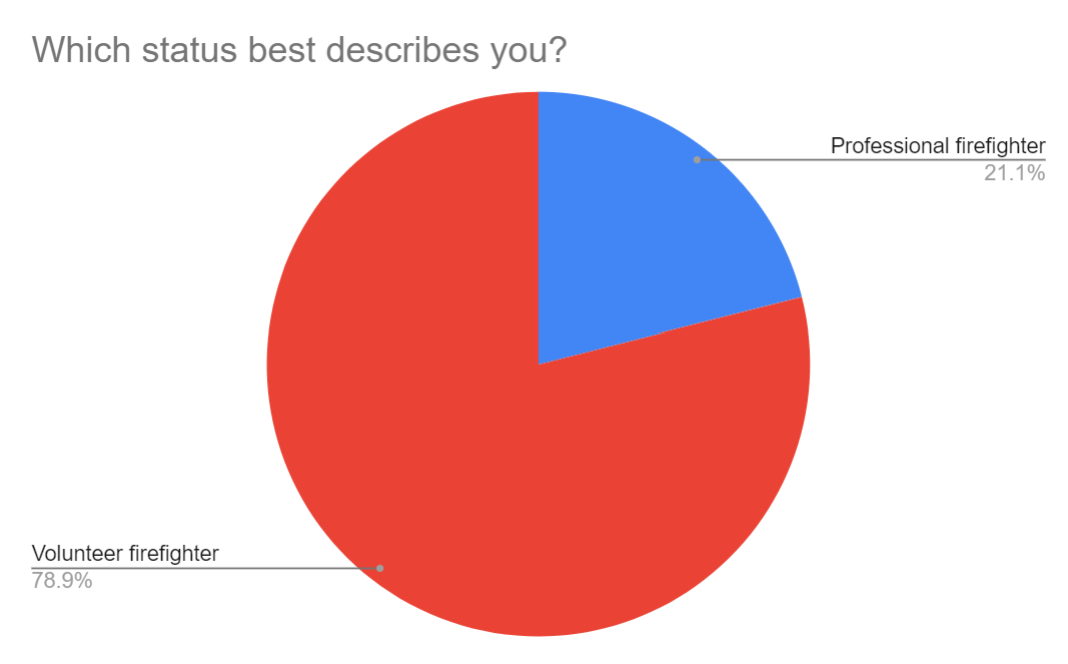
\includegraphics[width=11cm]{survey_graph_status}
  \caption{Verteilung des Berufsstatus}
  \label{fig:survey_graph_status}
\end{figure}

\begin{figure}[H]
  \centering
  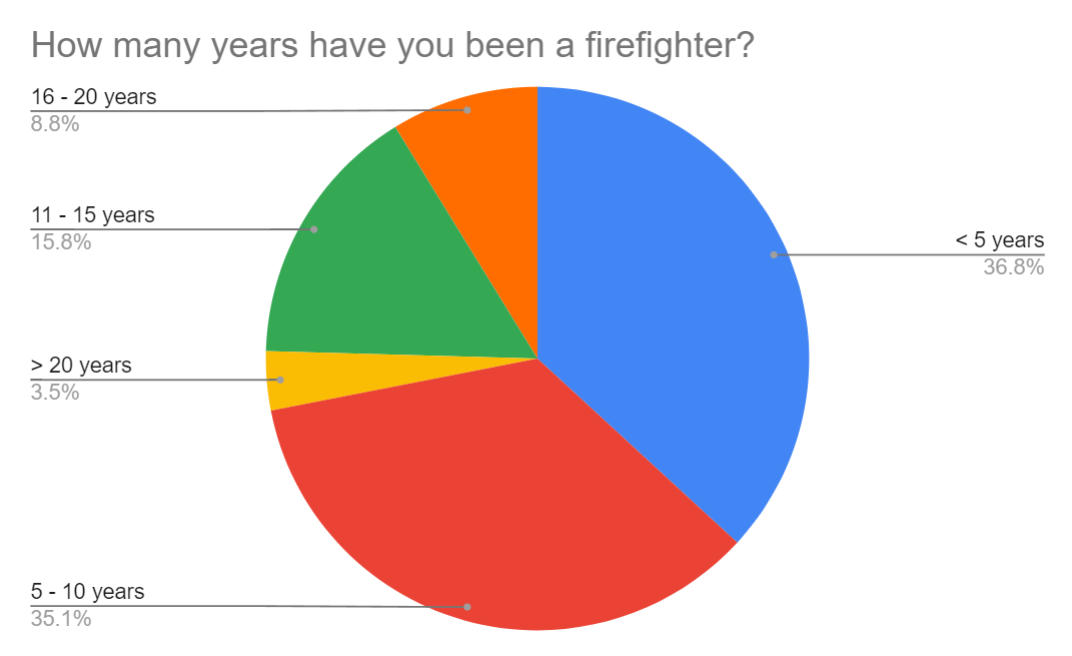
\includegraphics[width=11cm]{survey_graph_years}
  \caption{Verteilung der Dienstjahre}
  \label{fig:survey_graph_years}
\end{figure}

\begin{figure}[H]
  \centering
  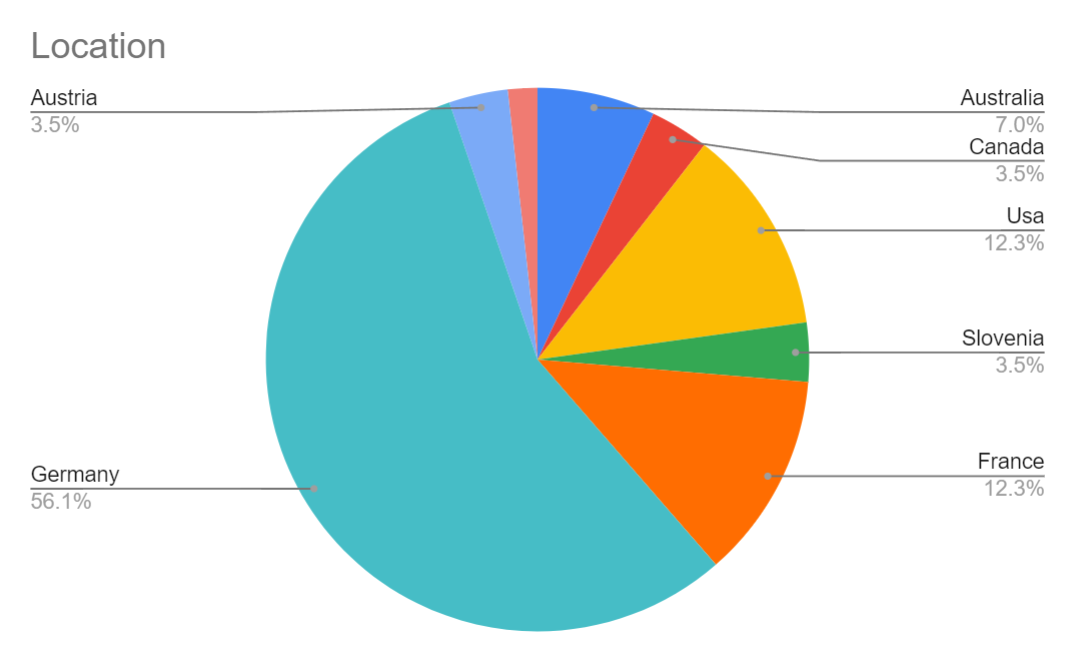
\includegraphics[width=11cm]{survey_graph_location}
  \caption{Geografische Verteilung der Antworten des Fragebogens}
  \label{fig:survey_graph_location}
\end{figure}

\begin{figure}[H]
  \centering
  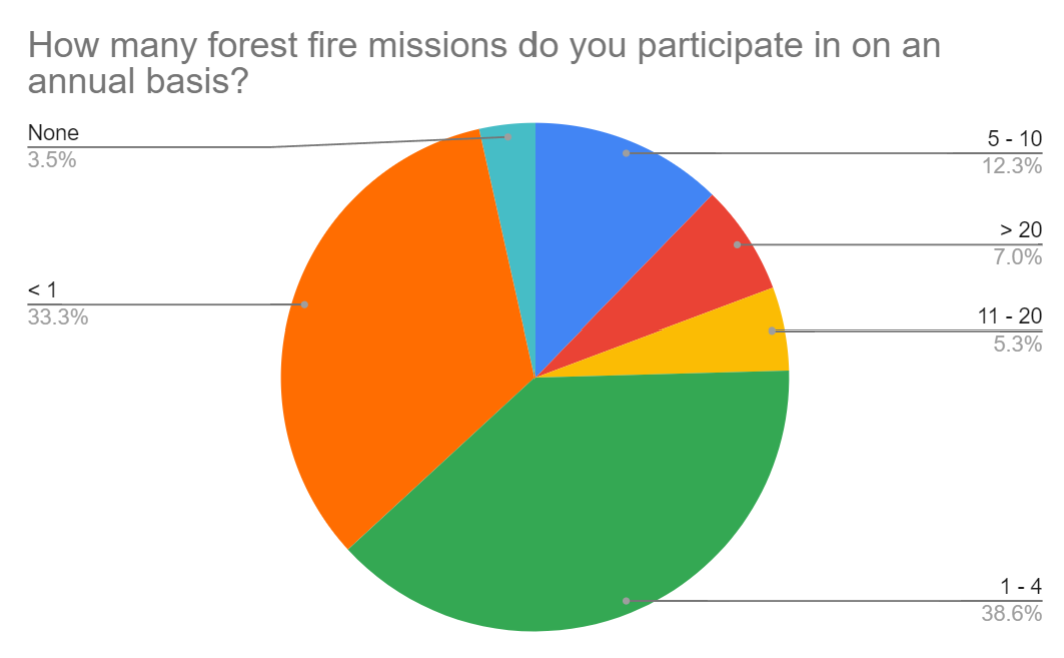
\includegraphics[width=11cm]{survey_graph_missions}
  \caption{Verteilung der durchschnittlich beteiligten Waldbrandeinsätze im Jahr}
  \label{fig:survey_graph_missions}
\end{figure}

\begin{figure}[H]
  \centering
  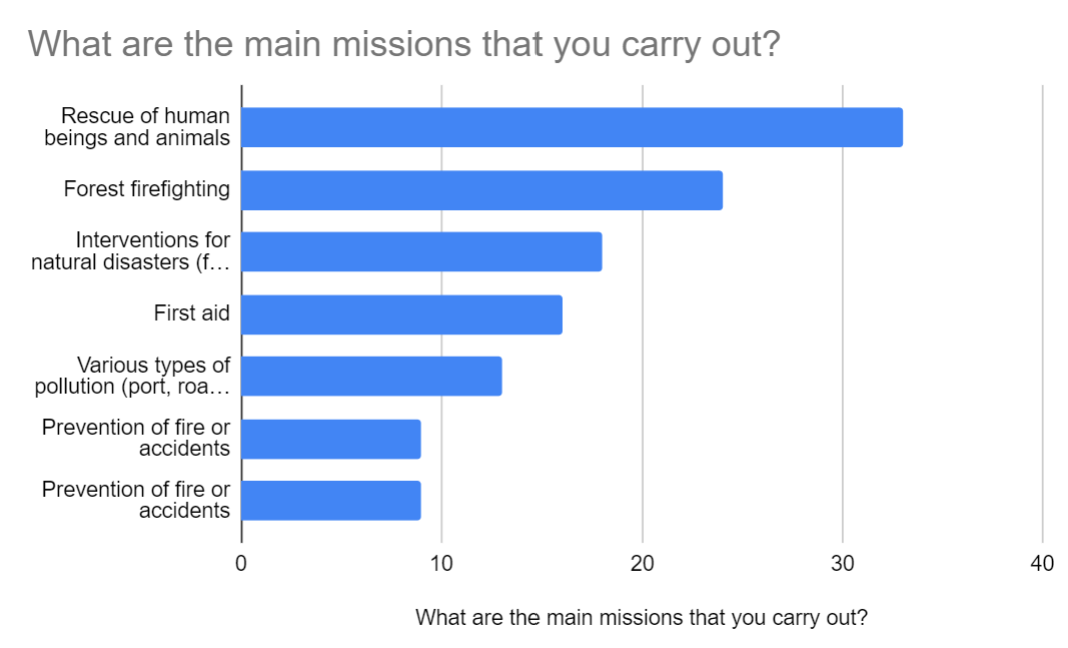
\includegraphics[width=11cm]{survey_graph_main_missions}
  \caption{Verteilung der verschiedenen Aufgaben, die hauptsächlich während des Dienstes erledigt werden}
  \label{fig:survey_graph_main_missions}
\end{figure}

\begin{figure}[H]
  \centering
  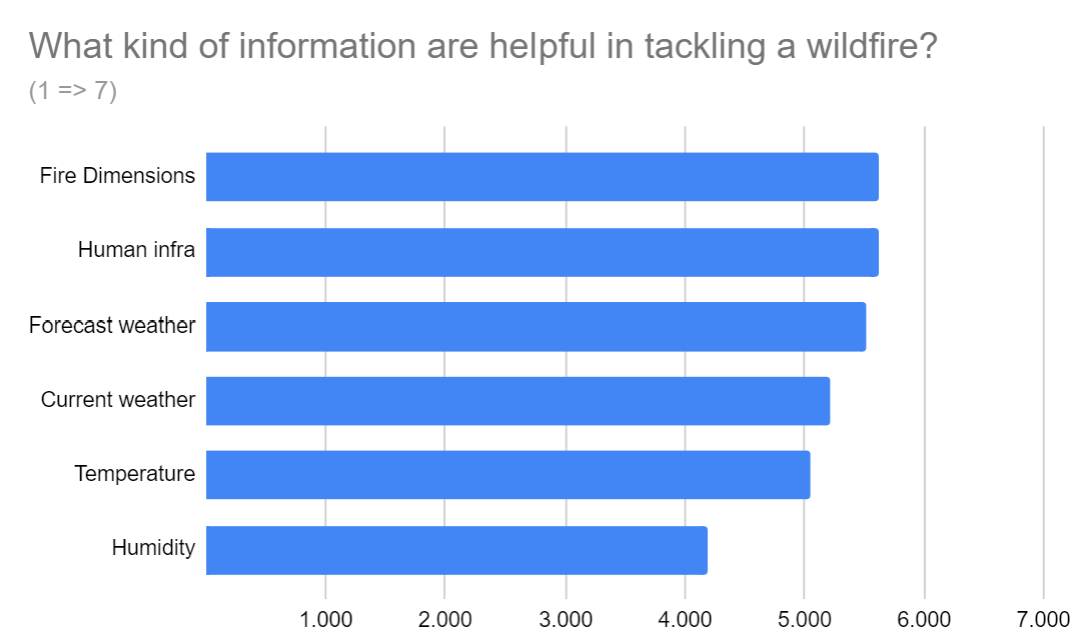
\includegraphics[width=11cm]{survey_graph_tackling}
  \caption{Relevanz der Daten zur Bekämpfung eines Waldbrandes}
  \label{fig:survey_graph_tackling}
\end{figure}

\begin{figure}[H]
  \centering
  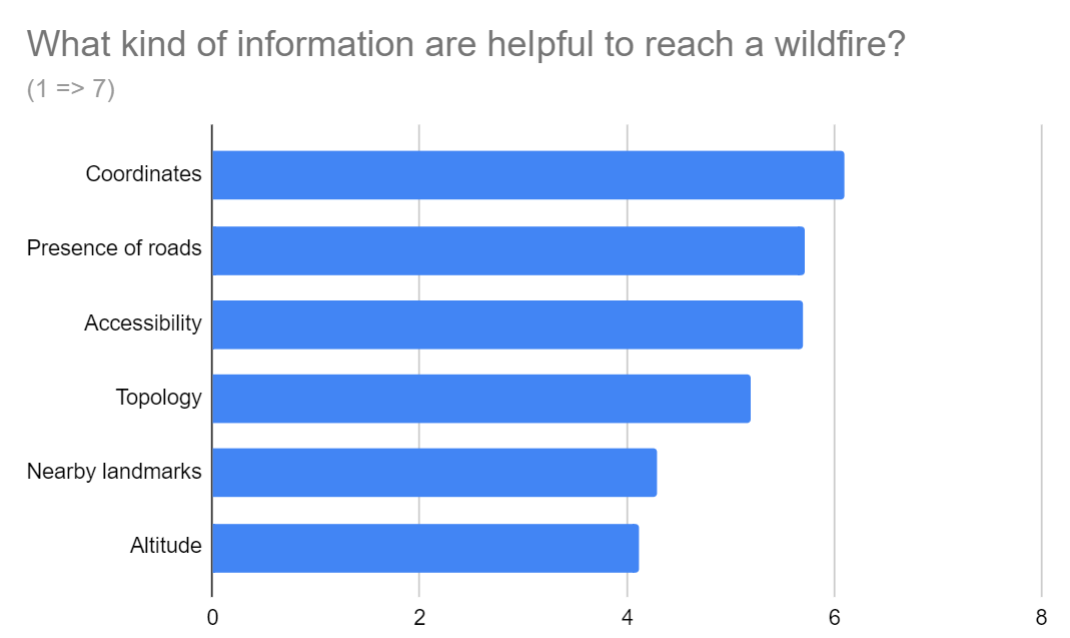
\includegraphics[width=11cm]{survey_graph_reach_fire}
  \caption{Relevanz der Daten, die den Zugang zu einem Waldbrand ermöglichen}
  \label{fig:survey_graph_reach_fire}
\end{figure}

\begin{figure}[H]
  \centering
  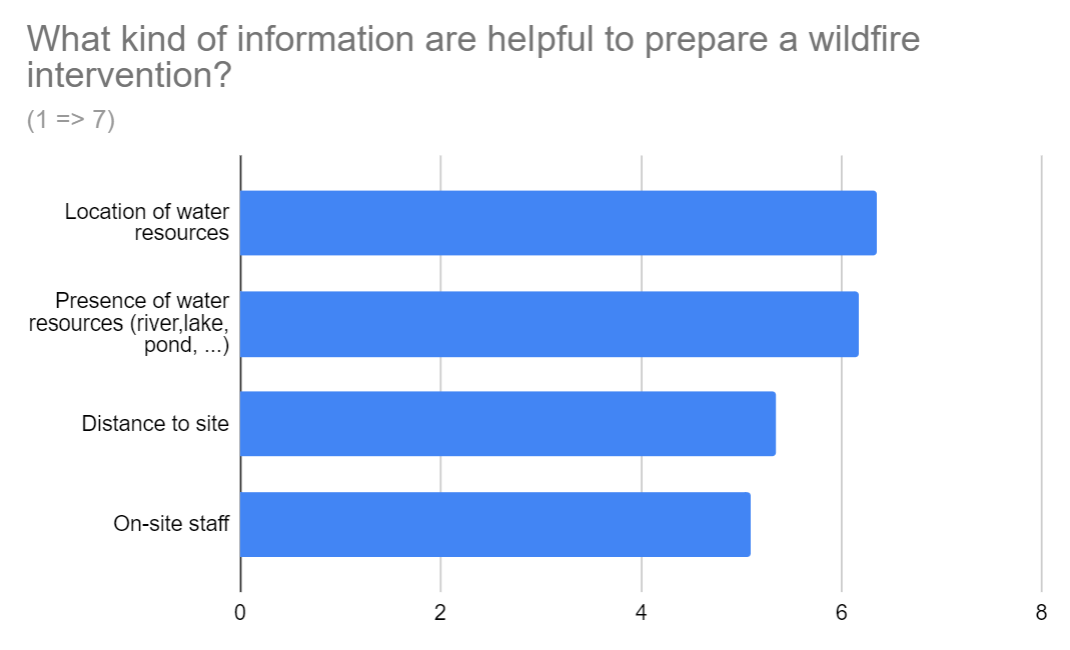
\includegraphics[width=11cm]{survey_graph_prepare}
  \caption{Relevanz der Daten zur Vorbereitung eines Feuerwehreinsatzes}
  \label{fig:survey_graph_prepare}
\end{figure}

\begin{figure}[H]
  \centering
  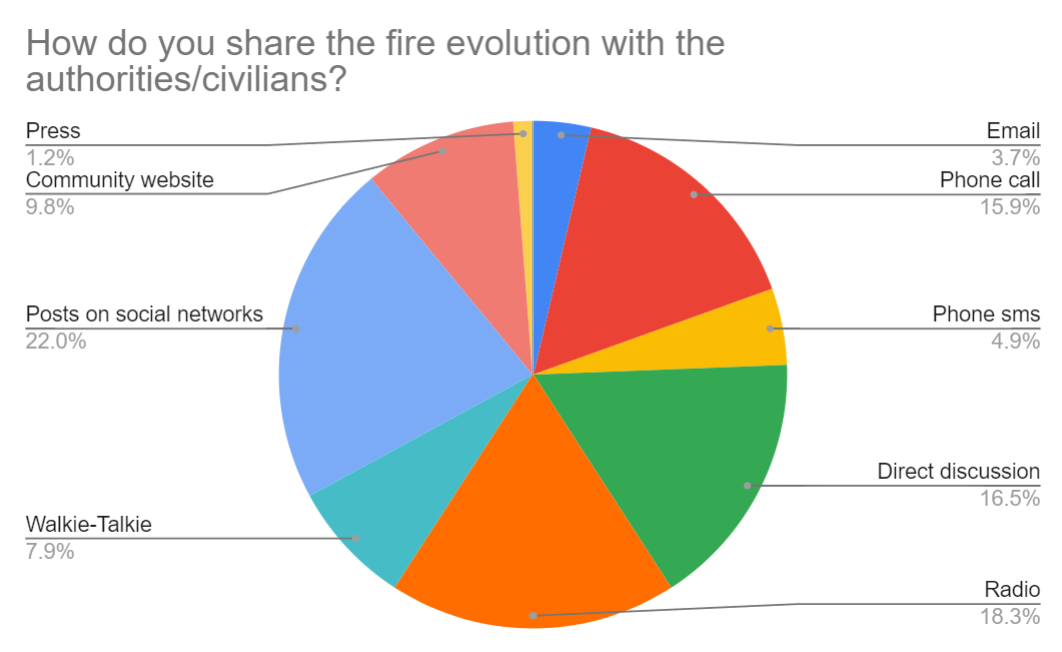
\includegraphics[width=11cm]{survey_graph_share_evolution}
  \caption{Verteilung der Methoden, die verwendet werden, um die Entwicklung eines Waldbrandes mitzuteilen}
  \label{fig:survey_graph_share_evolution}
\end{figure}

\begin{figure}[H]
  \centering
  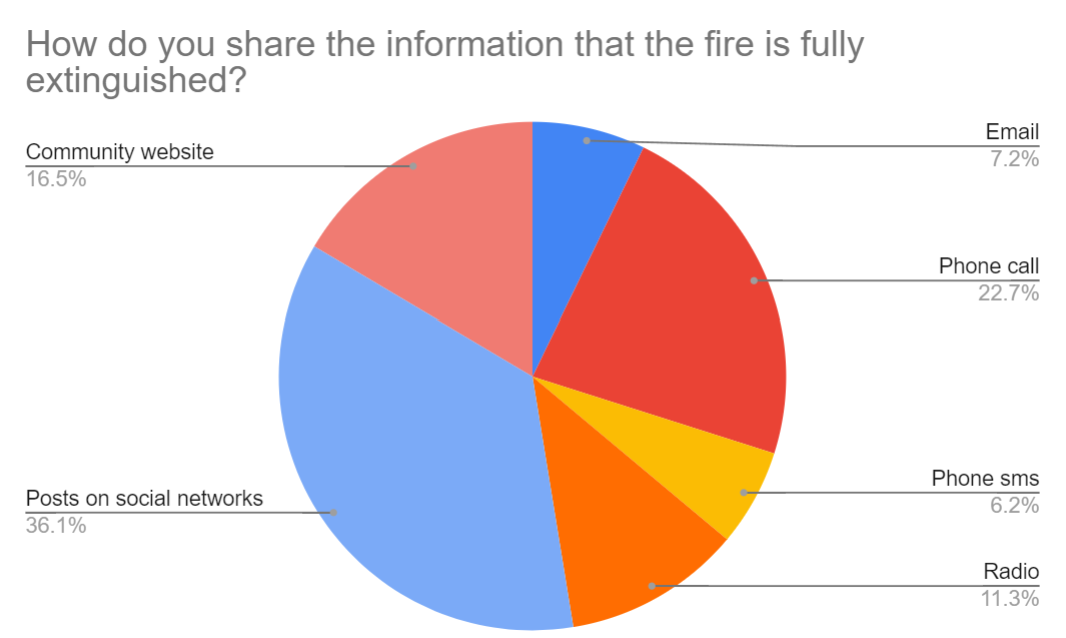
\includegraphics[width=11cm]{survey_graph_share_extinction}
  \caption{Verteilung der Methoden, mit denen die Nachricht vom Löschen eines Waldbrandes geteilt wird}
  \label{fig:survey_graph_share_extinction}
\end{figure}

\begin{figure}[H]
  \centering
  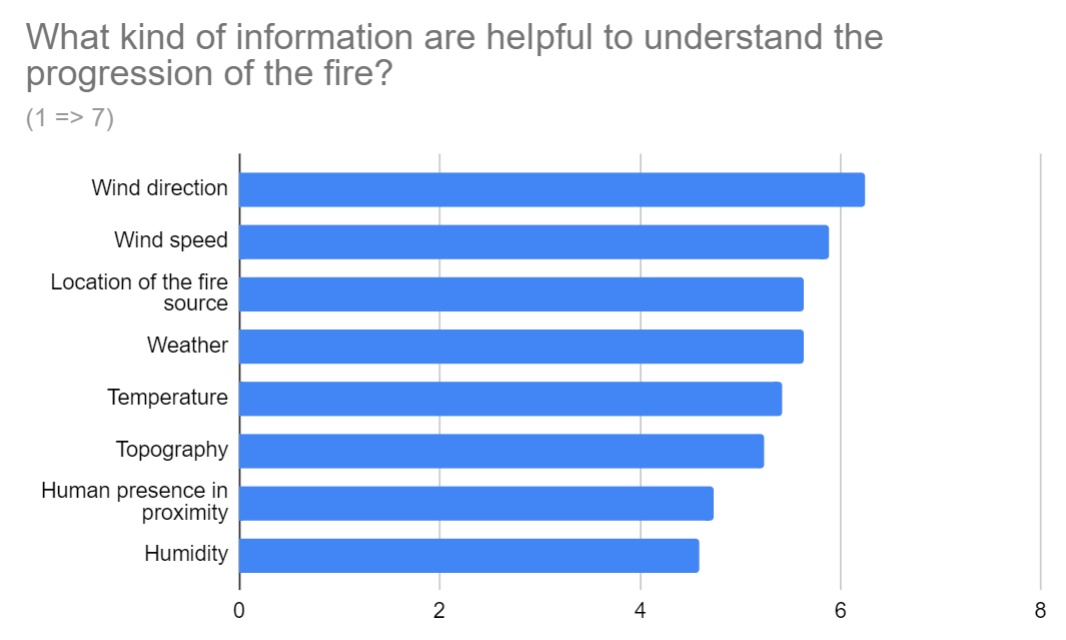
\includegraphics[width=11cm]{survey_graph_progression}
  \caption{Relevanz der Daten zum Verständnis der Entwicklung eines Waldbrands}
  \label{fig:survey_graph_progression}
\end{figure}

\begin{figure}[H]
  \centering
  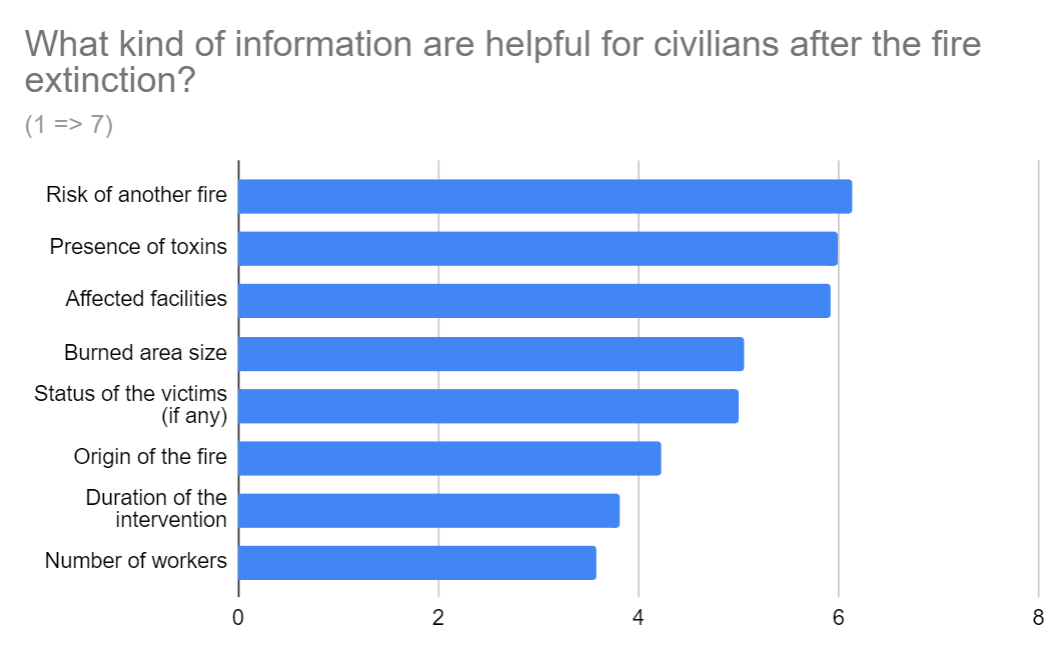
\includegraphics[width=11cm]{survey_graph_infos_civilians}
  \caption{Relevanz der Daten, die nach dem Löschen eines Waldbrandes mit Zivilisten geteilt werden sollen}
  \label{fig:survey_graph_infos_civilians}
\end{figure}

\begin{figure}[H]
  \centering
  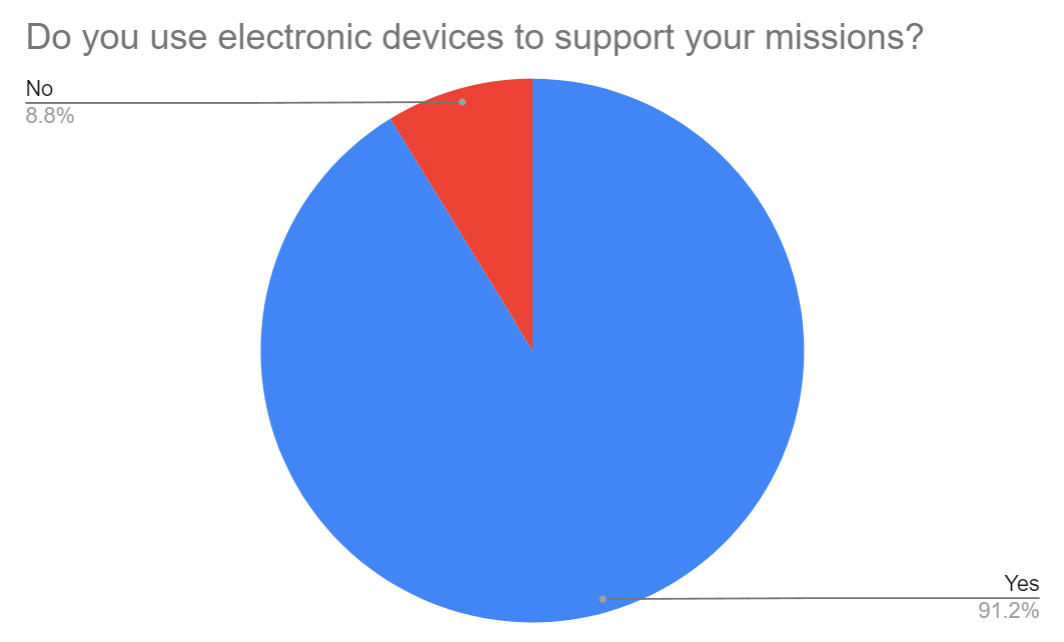
\includegraphics[width=11cm]{survey_graph_use_devices}
  \caption{Verteilung der Feuerwehrleute, die elektronische Geräte zur Unterstützung ihrer Arbeit verwenden}
  \label{fig:survey_graph_use_devices}
\end{figure}

\begin{figure}[H]
  \centering
  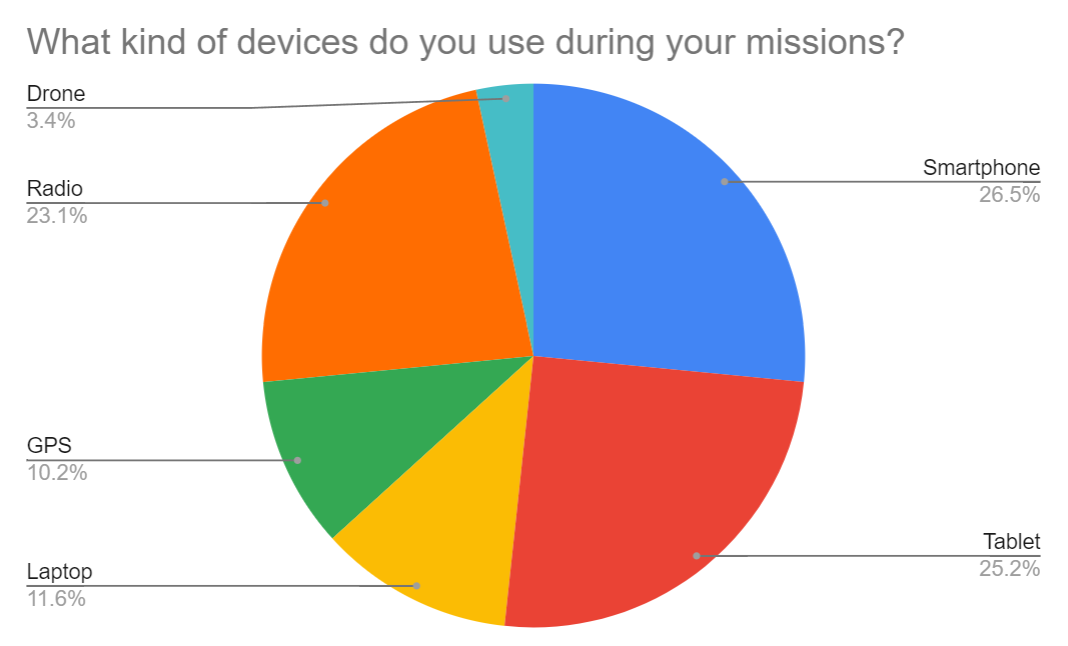
\includegraphics[width=11cm]{survey_graph_devices_mission}
  \caption{Verteilung der Arten von Elektrogeräten, die bei den Missionen verwendet wurden}
  \label{fig:survey_graph_devices_mission}
\end{figure}

\begin{figure}[H]
  \centering
  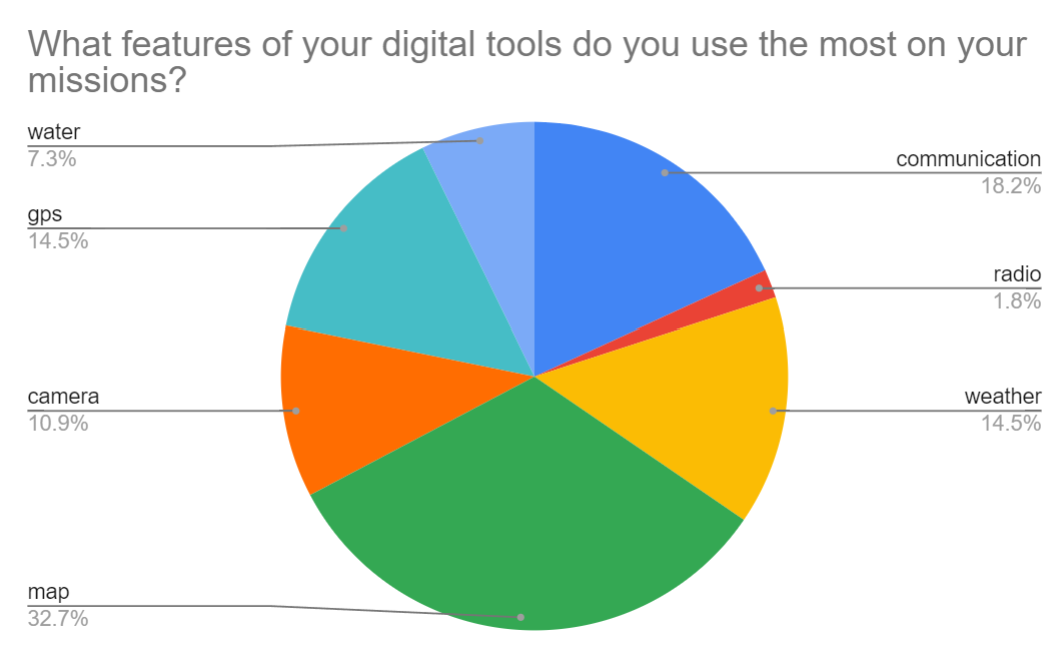
\includegraphics[width=11cm]{survey_graph_device_features}
  \caption{Verteilung der Funktionalität, die während der Missionen elektronische Geräte benutzte}
  \label{fig:survey_graph_device_features}
\end{figure}

\begin{figure}[H]
  \centering
  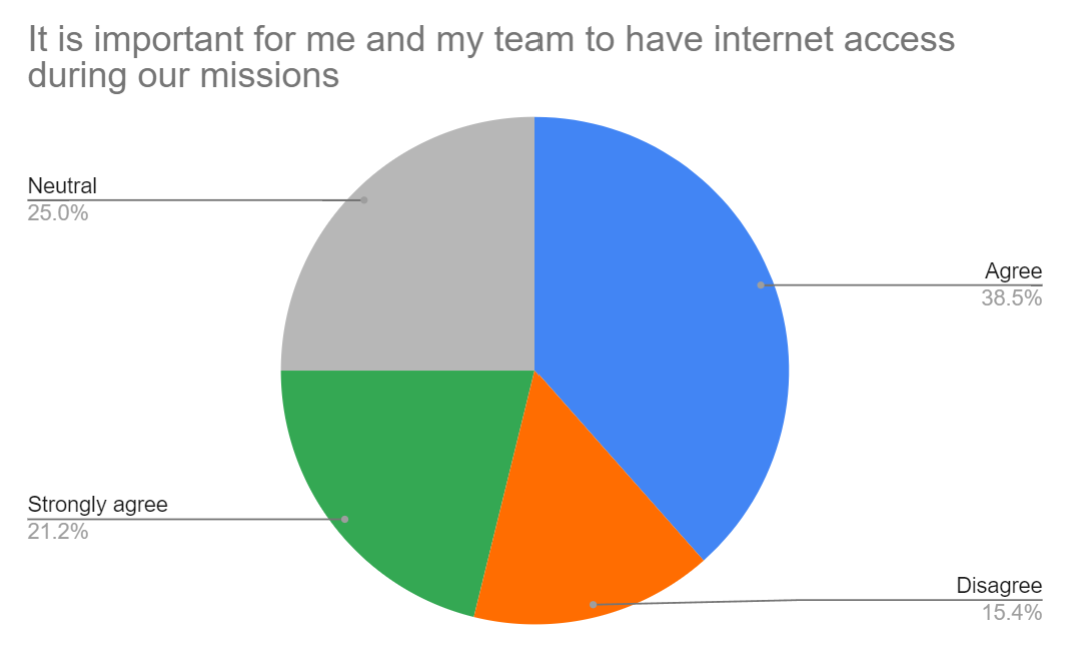
\includegraphics[width=11cm]{survey_graph_internet_missions}
  \caption{Verteilung der Internetnutzung während der Missionen}
  \label{fig:survey_graph_internet_missions}
\end{figure}

\begin{figure}[H]
  \centering
  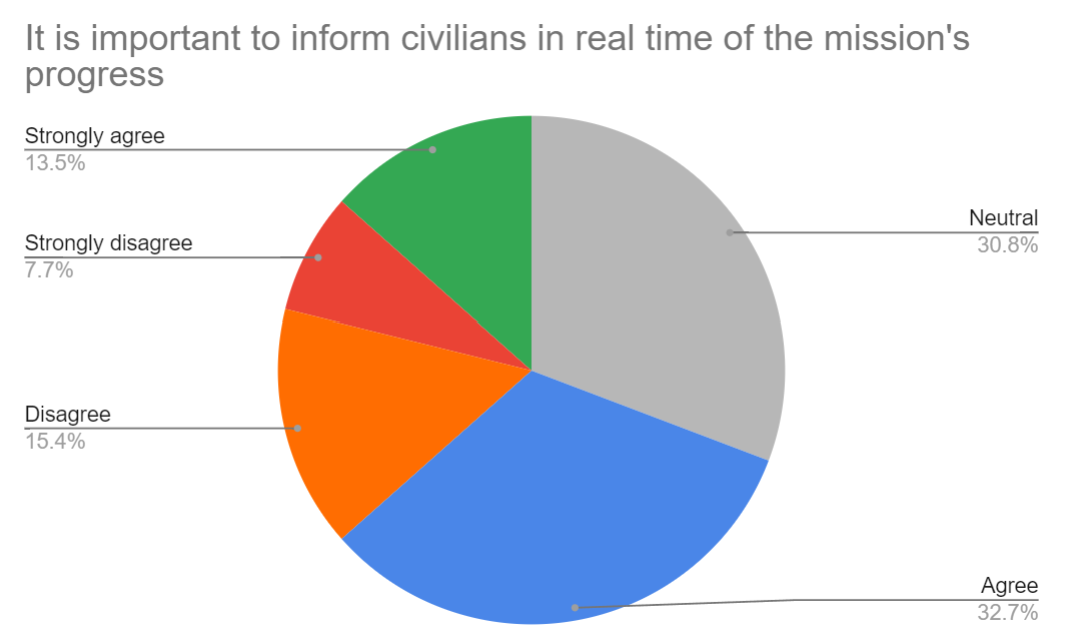
\includegraphics[width=11cm]{survey_graph_informcivilians}
  \caption{Relevanz der Information der Zivilbevölkerung über den Fortschritt der Mission zur Bekämpfung eines Waldbrandes}
  \label{fig:survey_graph_informcivilians}
\end{figure}

\begin{figure}[H]
  \centering
  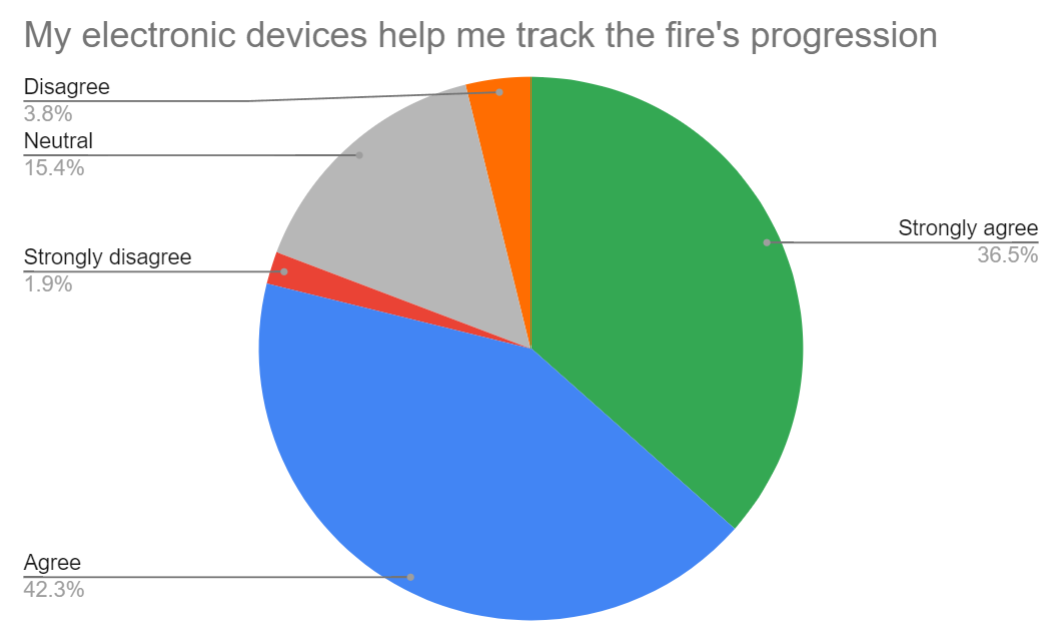
\includegraphics[width=11cm]{survey_graph_devices_helpfull}
  \caption{Relevanz von elektronischen Geräten für die Unterstützung bei der Überwachung der Ausbreitung eines Waldbrandes}
  \label{fig:survey_graph_devices_helpfull}
\end{figure}
